\documentclass[
  % -- opções da classe memoir --
  12pt,				% tamanho da fonte
  %openright,			% capítulos começam em pág ímpar (insere página vazia caso preciso)
  openany,
  %twoside,			% para impressão em verso e anverso. Oposto a oneside
  oneside,
  %titlepage,
  a4paper,			% tamanho do papel.
  % -- opções da classe abntex2 --
  %chapter=TITLE,		% títulos de capítulos convertidos em letras maiúsculas
  %section=TITLE,		% títulos de seções convertidos em letras maiúsculas
  %subsection=TITLE,	% títulos de subseções convertidos em letras maiúsculas
  %subsubsection=TITLE,% títulos de subsubseções convertidos em letras maiúsculas
  % -- opções do pacote babel --
  english,			% idioma adicional para hifenização
  brazil
]{article}
\usepackage[utf8]{inputenc}
\usepackage[brazil]{babel}
\usepackage{amsfonts}
\usepackage{indentfirst}
\usepackage[T1]{fontenc}
\usepackage{helvet}
\renewcommand{\familydefault}{\sfdefault}
\usepackage[left=3cm, right=2cm, top=3cm, bottom=2cm]{geometry}
\usepackage{setspace}
\usepackage{epigraph}
\usepackage{graphicx}
\usepackage{hyperref}
\usepackage{amsmath}
\numberwithin{figure}{section}
\numberwithin{table}{section}

\graphicspath{{figuras/}}

\renewcommand{\baselinestretch}{1.5}
\setlength{\parindent}{3em}
\setlength{\parskip}{1em}

%% DEFINEs dos textos constantes da capa
\newcommand{\defUFABC}{UNIVERSIDADE FEDERAL DO ABC}
\newcommand{\defBCC}{BACHARELADO EM CIÊNCIA DA COMPUTAÇÃO}
\newcommand{\defRelatorio}{RELATÓRIO DO ESTÁGIO SUPERVISIONADO I} %%ESTÁGIO SUPERVISIONADO
\newcommand{\defTitulo}{ESTÁGIO EM DESENVOLVIMENTO DE SISTEMA PARA USO INTERNO NA AGÊNCIA CADARIS}
\newcommand{\defRafael}{RAFAEL CARDOSO DA SILVA}
\newcommand{\defOrientador}{Orientador: Prof. Dr. Daniel Morgato Martin}
\newcommand{\defLocaldata}{Santo André, 2017}

\begin{document}

%%--[ELEMENTOS PRÉ-TEXTUAIS]--%%

%%--CAPA--%%

\begin{titlepage}

\begin{center}
\text{ \defUFABC }
\text{ \defBCC }\\\vspace{5cm}
\textbf{\large{ \defRelatorio }}\\\vspace{4cm}
\textbf{\Large{\defTitulo}}\\\vspace{4cm}
% Nome do Autor
\textbf{\large{ \defRafael }}\\\vspace{2cm}
% Orientador
\textbf{\large{ \defOrientador }}\\\vspace{3cm}
\textbf{\defLocaldata}
\end{center}

\end{titlepage}

%%--FOLHA DE ROSTO--%%

\begin{titlepage}

\begin{center}
\textbf{\large{ \defRafael }}\\\vspace{6cm}
\textbf{\Large{ \defTitulo }}\\\vspace{5cm}
\begin{raggedleft}{
Relatório do Estágio apresentado ao Curso de\\
Bacharelado em Ciência da Computação como\\
requisito parcial para obtenção do grau de\\
Bacharel em Ciência da Computação
\\\vspace{1cm}

%  Trabalho apresentado à banca de Estágio\\
%  Supervisionado como requisito parcial para\\
%  obtenção do título de Bacharel em Ciência da\\
%  Computação pela Universidade Federal do ABC.\\
\large{ \defOrientador }
}\\\vspace{5cm}
\end{raggedleft}
\textbf{ \defLocaldata }
\end{center}

\end{titlepage}

%%--DEDICATÓRIA--%%

\begin{titlepage}

\begin{center}
\textbf{DEDICATÓRIA}
\end{center}

Dedico todo projeto realizado aos meus amigos e familiares que depositaram grande confiança em mim desde o início.


\end{titlepage}

%%--AGRADECIMENTOS--%%

\begin{titlepage}

\begin{center}
\textbf{AGRADECIMENTOS}
\end{center}

Meus agradecimentos são voltados à Agência Cadaris, principalmente a Diretoria Comercial, que propôs essa oportunidade de amadurecer meus conhecimentos obtidos na Universidade Federal do ABC, além do crescimento pessoal.


\end{titlepage}

%%--EPÍGRAFE--%%

\begin{titlepage}


.\\\vspace{18cm}
\begin{raggedleft}

\begin{epigraph} {????????????????????? \\A maioria das pessoas pensa no sucesso e no fracasso como opostos, mas eles são ambos produtos do mesmo processo}{Roger Von Oech}

\end{epigraph}
\end{raggedleft}

\end{titlepage}

%%--RESUMO--%%

\begin{titlepage}

\begin{center}
\textbf{RESUMO}
\end{center}

% TODO: RESUMO

????????????????? DEPOIS ?????????????????

%O estágio consiste na manutenção de sistemas existentes em PHP, tanto nas permissões de acesso de usuários quanto segurança das informações. Geralmente são correções e adição de informações nas funcionalidades já existentes. Novos sistemas são desenvolvidos com o framework .NET, banco de dados SQL Server e padrão MVC. A fim de melhorar a experiência do desenvolvimento e do usuário final, ferramentas modernas são exploradas, como o AngularJS by Google. O sistema de bolsa de estudos foi o primeiro com a ferramenta e, após êxito no desenvolvimento e nos testes, foi iniciado o sistema de gerenciamento de projetos com exploração máxima dos recursos, com mais agilidade e padrão no desenvolvimento e uma experiência mais ativa e dinâmica por parte do usuário final.


\end{titlepage}

%%--ABSTRACT--%%

\begin{titlepage}

\begin{center}
\textbf{ABSTRACT}
\end{center}
% TODO: RESUMO ingles

????????????????? DEPOIS ?????????????????

%The internship is the maintenance of existing systems in PHP, both on user access permissions as information security. Usually fixes and adding information to existing functionality. New systems are developed with the .NET framework, SQL Server database and MVC pattern. To enhance the experience of development and user, modern tools are explored, such as angularjs by Google. The scholarship system was the first with the tool and, after successful development and testing, started the project management system with maximum exploitation of resources, more quickly and standard development and a more active and dynamic experience by the user.


\end{titlepage}


%%%--LISTA DE FIGURAS--%%
%
%\begin{titlepage}
%
%\begin{center}
%  \begin{singlespace}
%    \listoffigures
%  \end{singlespace}
%\end{center}
%
%\end{titlepage}


%%--SUMÁRIO--%%

\begin{titlepage}

\begin{center}
  \begin{singlespace}
    \tableofcontents
  \end{singlespace}
\end{center}

\end{titlepage}


%%--[ELEMENTOS TEXTUAIS]--%%

\section{INTRODUÇÃO}

O estágio é uma atividade fundamental para a formação do aluno que está matriculado em um curso de nível superior. Nessa atividade o aluno tem a possibilidade de aplicar o conhecimento adquirido durante o período de graduação, além de poder desenvolver novos conhecimentos e habilidades ao enfrentar novos desafios e buscar soluções para problemas corriqueiros do trabalho realizado dentro de uma empresa.

Também é de muita importância para o desenvolvimento pessoal e profissional do aluno, visto que é o primeiro contato com o mercado de trabalho. Isso permite que o aluno desenvolva mais responsabilidades e aprenda a trabalhar em equipe, além de aprender a lidar com problemas reais dentro de uma empresa.

O estágio é uma tarefa supervisionada por um orientador e é gerado um relatório que é utilizado para se fazer a avaliação do aluno durante a atividade do estágio.

Este relatório tem por objetivo descrever as atividades e os produtos obtidos durante a disciplina de Estágio Supervisionado I. Nesta seção, apresenta-se a caracterização do estágio, da empresa, uma visão geral do estágio e a organização geral deste documento.


\subsection{CARACTERÍSTICAS DO ESTÁGIO}

A modalidade deste estágio é em \textit{Home Office}\footnote{Escritório em casa, em uma tradução livre do inglês, trabalho que é realizado em espaço alternativo ao escritório de uma empresa.}, que também pode ser definido com um trabalho remoto ou teletrabalho, para a Agência Cadaris \textit{[ref:Cadaris]}. A jornada de trabalho é de segunda à sexta-feira, desemprenhando 6 horas diárias, totalizando 30 horas semanais, com a gratificação de uma bolsa de R\$ 1.100,00 por mês.

A função principal deste estágio é o desenvolvimento de um projeto de uso interno para a empresa. E por se tratar de um \textit{Home Office}, proporcionando ao aluno um horário mais flexível de trabalho, como melhor se adapte a sua agenda acadêmica e pessoal. E também mantem a comunicação direta com a empresa por meio de e-mails e ligações via telefone e \textit{Skype}.



\subsection{CARACTERIZAÇÃO E ANÁLISE DA EMPRESA}

%  A Cadaris é uma agência de publicidade com atuação nas áreas de marketing, editorial e comunicação. Aqui, trabalho em equipe é lei e surpreender o cliente, uma meta diária.
%  Trabalhamos com ética e transparência, de forma responsável e comprometida. Produzimos com qualidade e criatividade, sempre com respeito aos prazos acordados.
%  Queremos ser reconhecidos como uma agência diferenciada, por clientes e funcionários.
%  Entre os nossos principais clientes estão: Colgate-Palmolive, Biotropic, ABO, TAM e Mattel, entre outras empresas.
%  Para saber mais sobre a Cadaris, acesse www.cadaris.com.br ou envie um email para cadaris@cadaris.com.br

%  Products:
%    Publicidade: anúncios, materiais de ponto de venda, materiais promocionais, apresentações de produtos e campanhas, hotsites, etc.
%    Comunicação: campanhas dirigidas e campanhas de comunicação interna
%    Editorial: revistas, informativos, enews, jornal-mural, guias e relatórios, manuais, cartilhas, etc.



O estágio foi iniciado no dia 01/08/2016, contratado pela Agência Cadaris, CNPJ 01.556.009/0001-46, que é uma agência de publicidade e está localizada na R. Dr. Thirso Martins, 100, cj 303, CEP:~04120-050, Vila Mariana, São Paulo-SP, telefone:~(11)~5571-9142.

Cadaris foi fundada.....

A Agência Cadaris é uma agência de publicidade com atuação nas áreas de marketing, editorial e comunicação. Trabalhando com ética e transparência, de forma responsável e comprometida. Produzindo com qualidade e criatividade, sempre com respeito aos prazos acordados.

A empresa é formada por...

Os principais clientes da Cadaris estão: Colgate-Palmolive, Biotropic, ABO, TAM e Mattel, entre outras empresas.



\subsection{VISÃO GERAL DO ESTÁGIO}


Inicialmente, durante o primeiras mês, o estagiário foi introduzido ao funcionamento da agência, com a familiarização das regras de negócio e as ferramentas atuais utilizadas para apoiar a administração da empresa.

Após este período inicial, foi iniciada o estudo das tecnologias que serão utilizadas para o desenvolvimento deste sistema, que foi completamente discutido no período anterior.

A seguir é iniciado a implementação do sistema após todos os estudos e os planejamentos deste, com foco no \textit{Back-end}. Primeiramente é desenvolvido o Cadastro de recursos e algumas rotinas administrativas. Em seguida o processo Comercial. E por ultimo a geração de Relatórios e controle Financeiro.

Ao final é desenvolvido um novo \textit{Front-end} para o sistema, junto ao time de \textit{Front-end} da Cadaris, com recursos necessários para uma melhor experiência do usuário.

%Após o período de integração, foi iniciado o principal projeto do estágio: Sistema de Gestão de Atividades. Esse projeto possui várias características de um grande sistema e exigiu conhecimentos acadêmicos específicos, como: banco de dados, orientação à objetos, programação para web, planejamento e estruturação.

%Após um mês de desenvolvimento do Sistema de Gestão de Atividades, foi iniciado o projeto Sistema de Bolsa de Estudos PROMAIS, a fim de testar novas ferramentas que poderiam ser utilizadas no primeiro citado. O Sistema de Bolsa de Estudos PROMAIS demorou dois meses para ser finalizado e então foi iniciado novamente o Sistema de Gestão de Atividades, dessa vez com as novas ferramentas testadas e introduzidas. O projeto permanece em desenvolvimento durante a elaboração deste relatório.


\subsection{ORGANIZAÇÃO DO TRABALHO}

As próximas seções estão organizadas como segue:

A seção 2 apresenta as informações detalhadas de todas as atividades realizadas pelo estagiário. A seção está dividida em quatro partes, uma para cada atividade desenvolvida.

A seção 3 descreve as considerações finais em relação a todo o estágio, como: contribuições para a formação, dificuldades encontradas e sugestões para trabalhos futuros.

A seção 4 apresenta os principais problemas observados pelo estagiário em cada etapa e sugestões de melhorias para cada uma delas.

A seção 5 detalha a relação entre as disciplinas cursadas pelo estagiário e as atividades realizadas durante os projetos.

A seção 6 apresenta a conclusão sobre o estágio desenvolvido.






\section{ATIVIDADES DESENVOLVIDAS}

%%--Descrever as atividades realizadas no estágio--%%

Esta seção tem por objetivo detalhar as atividades desenvolvidas durante o estágio supervisionado. Inicialmente são apresentadas as atividades de aprendizagem e em seguida a de desenvolvimento.


\noindent \texttt{
  Lista de trabalhos realizados:\\
  ESTÁGIO 1 \\
  - Reunião sobre as regras de negócio da empresa (DER) \\
  - Estudo das tecnologias a serem utilizados (Laravel, bootstrap) \\
  - Dev o sistema para substituir a antes utilizada (antigo: planilhas) \\
  ESTÁGIO 2 \\
  - Dev o sistema conforme as regras de negocio atual da empresa (antigo: VBD) \\
  - Dev o sistema para a geração de relatórios e controle financeiro \\
  ESTÁGIO 3 \\
  - Front-end (VueJS) \\
  - teste, homologacao, e ajuste finais \\
  - Outras áreas da empresa
}


\subsection{APRESENTAÇÃO DAS REGRAS DE NEGÓCIO}

\subsection{ESTUDO DAS TECNOLOGIAS DE DESENVOLVIMENTO WEB}

\subsection{IMPLEMENTAÇÃO}

  \subsubsection{CADASTROS}
  
  \subsubsection{COMERCIAL}
  
  \subsubsection{RELATÓRIOS E CONTROLE FINANCEIRO}


\subsection{INTERFACE E EXPERIÊNCIA DE USUÁRIO}

\subsection{HOMOLOGAÇÃO, E AJUSTE FINAIS}

\subsection{OUTRAS ÁREAS DA EMPRESA}



\subsubsection{Resultados}
\subsubsection{Conclusão}



\subsection{DIAGNÓSTICO DOS PRINCIPAIS PROBLEMAS OBSERVADOS E SUGESTÕES DE MELHORIA}


%Os sistemas em PHP são de longa data e poderiam ser desenvolvidas novas versões com mais funcionalidades e layout responsivo. Existem famosos CMS em PHP que poderiam trazer benefícios aos sistemas, como o Wordpress, ou então a utilização de algum framework, como o Zend.

%O sistema de Bolsa de Estudos PROMAIS era muito antigo e desenvolvido em Microsoft Access, ou seja, muito defasado e impróprio para a utilização em uma empresa. A solução foi o desenvolvimento de um novo sistema desde o início com o Microsoft Visual Studio, C\#, AngularJS, SQL Server e orientação à objetos. Algumas implementações ainda podem ser realizadas como perfis de usuários e permissões, especificando que alguns usuários possam editar e outros apenas visualizar as informações.

%O Sistema de Gestão de Atividade teve um grande avanço entre as duas primeiras versões. Novas funcionalidades foram inseridas devido às novas ferramentas e tem grande potencial. Melhorias podem ser inseridas, como: novos filtros, edição de comentários, gráficos dinâmicos, sistema de notificações locais e por e-mail, perfis de usuários com permissões por setor e individual.



\section{FUNDAMENTAÇÃO TEÓRICA}

%%-- Descrever as disciplinas utilizadas e dar exemplos--%%


As disciplinas cursadas contribuíram de várias formas, direta ou indiretamente, nas atividades realizadas no período de estágio. A Tabela 3.1 apresenta as disciplinas cursadas pelo aluno e que foram necessárias para o desenvolvimento das atividades.

\begin{table}[!htb]
\centering
\caption{Disciplinas desenvolvidas durante o estágio com os suas respectivas abordagens.
}
\begin{tabular}{|c|l|}
\hline
Algoritmo e estrutura de dados       & Ordenação                                                                                                                                        \\ \hline
Análise de algoritmos                & Custo de operações                                                                                                                               \\ \hline
Banco de dados                       & \begin{tabular}[c]{@{}l@{}}Banco de dados relacional;\\ Diagrama Entidade-Relacionamento;\\ Diagrama de classes;  \\ Consultas SQL.\end{tabular} \\ \hline
Engenharia de software               & \begin{tabular}[c]{@{}l@{}}Planejamento; \\ Modelo Entidade-Relacionamento; \\ Padrão MVC.\end{tabular}                                          \\ \hline
Linguagens formais e autômata        & Expressões Regulares.                                                                                                                            \\ \hline
Lógica básica                        & Operadores Lógicos                                                                                                                               \\ \hline
Processamento da informação          & Lógica de programação                                                                                                                            \\ \hline
Programação orientada a objetos      & Paradigma orientado a objetos.                                                                                                                   \\ \hline
Programação para Dispositivos Móveis & \begin{tabular}[c]{@{}l@{}}HTML;  \\ Responsividade\end{tabular}                                                                                 \\ \hline
Programação para Web                 & \begin{tabular}[c]{@{}l@{}}HTML; \\ CSS; \\ Javascript; \\ Servlet API.\end{tabular}                                                             \\ \hline
Segurança de Dados                   & \begin{tabular}[c]{@{}l@{}}Criptografia; \\ Autenticação.\end{tabular}                                                                           \\ \hline
\end{tabular}
\end{table}


\subsection{PLANEJAMENTO DE PROJETOS}


Segundo os pontos citados na Engenharia de Software e nos livros de Somerville \textit{[15]} e Pressman \textit{[16]}, não basta apenas programar e desenvolver projetos, é necessário ter um planejamento completo antes de iniciar a programação em si, além de possuir desenvolvedores competentes na equipe. Todo sistema está sujeito a falhas, mas quando há bom planejamento, incluindo os imprevistos, dificilmente terá grandes problemas durante o período de utilização, nada que o comprometa seriamente. Tais fatos foram notados ao desenvolver os sistemas de Bolsa de Estudos PROMAIS e Sistema de Gestão de Atividades. O primeiro foi totalmente planejado, desde a estrutura das classes como quais ferramentas seriam utilizadas e o projeto foi desenvolvido do começo ao fim como o previsto. O segundo projeto havia sido planejado, mas durante o desenvolvimento foi notada muita repetição de códigos e a necessidade de uma ferramenta que tornasse a aplicação mais dinâmica e suprisse esse obstáculo, e assim foi pesquisado e encontrado o AngularJS \textit{[4]}.




\subsection{DESENVOLVIMENTO WEB}

\subsubsection{HTML}

Em \textbf{Programação para Web} foram desenvolvidas aplicações para web e em \textbf{Programação para Dispositivos Móveis} foram vistos conceitos semelhantes ao HTML. O HTML5 é uma linguagem que foi desenvolvida para exibir conteúdos em páginas web. A diferença para algumas outras linguagens de programação é que o HTML5 não necessita ser compilado, ele é apenas interpretado pelo navegador. A programação é realizada através de tags (<tag>) que podem possuir atributos e elementos filhos, desde que estejam dentro da tag de fechamento, que é representada por uma barra (</tag>). A Figura 3.1 demonstra a estrutura de um arquivo HTML com algumas tags novas que foram introduzidas na versão 5, como header, nav, section, article, aside e footer. Novos elementos foram introduzidos para dar semântica à linguagem, ou seja, ao ler um código é possível ter noção do conteúdo que será apresentado de acordo com as tags utilizadas, nas versões anteriores, todo o conteúdo possuía o mesmo nível de informação.

\begin{figure}[!htb]
\centering
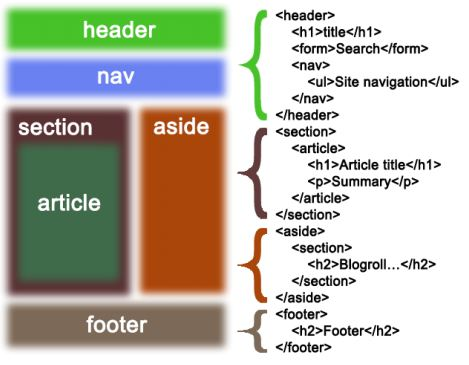
\includegraphics[width=0.6\textwidth]{figura31}
\caption{Estrutura do HTML com novas tags introduzidas na versão 5.}
\end{figure}

Com base na Figura 3.1, é demonstrada a herança de tags. As tags que são apresentadas dentro de uma tag de abertura e fechamento, são consideradas filhas, como h1, form e nav que são filhas da tag header.

O HTML5 é responsável pela exibição de conteúdo, sendo assim, não é capaz de criar novos elementos, conectar com um banco de dados ou com algum servidor, por exemplo. Essas outras atividades são realizadas por outras linguagens de programação que caminham em conjunto com o HTML5.



\subsubsection{JAVASCRIPT}


A linguagem de programação Javascript permite que haja interação entre o conteúdo HTML5 e o usuário, tornando a conteúdo da aplicação dinâmico. O DOM é uma multiplataforma que representa como as marcações em HTML, XHTML e XML são organizadas e lidas pelo navegador. Uma vez indexadas, estas marcações se transformam em elementos de uma árvore que você pode manipular via API, ou seja, o Javascript é capaz de manipular essas informações. Após o HTML ser carregado e interpretado pelo navegador, ele mesmo não tem poder para alterá-lo, mas o Javascript pode inserir, alterar ou remover nós em tempo de execução (Figura 3.2) \textit{[17]}.

\begin{figure}[!htb]
\centering
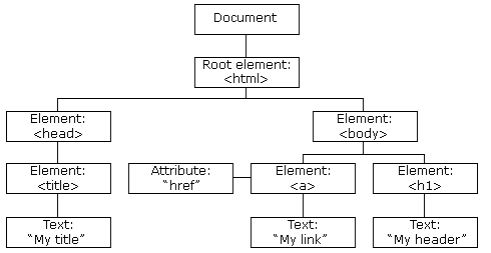
\includegraphics[width=1\textwidth]{figura32}
\caption{Estrutura de uma árvore DOM.}
\end{figure}

A Figura 3.3 apresenta um exemplo de manipulação de uma árvore DOM com o Javascript. A primeira linha cria uma tag do tipo “div” e salva na variável “el”. A segunda linha acrescenta a variável “el” ao elemento “body”. A terceira linha acrescenta uma classe CSS
“container” ao elemento “el”. A quarta linha adiciona uma margem superior de 30px ao elemento.
Se esse código fosse desenvolvido diretamente pelo HTML5, seria o mesmo que:
<body><div class=”container” style=”margin-top: 30px”></div></body>

\begin{figure}[!htb]
\centering
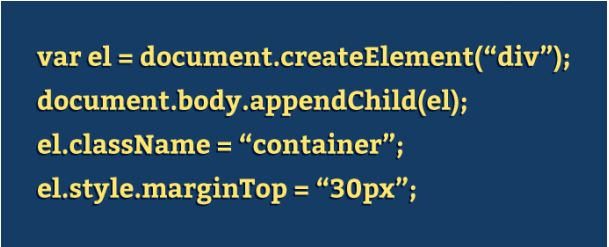
\includegraphics[width=1\textwidth]{figura33}
\caption{Exemplo de manipulação de DOM com Javascript.}
\end{figure}


\subsubsection{ANGULARJS}

O AngularJS \textit{[4]} foi o grande encarregado por essa função de manipular o DOM nos sistemas de Bolsa de Estudos PROMAIS e o de Gestão de Atividades. A única necessidade do desenvolvedor é se preocupar com o JSON gerado e o AngularJS \textit{[4]} o interpreta e cria o DOM de acordo com as informações que recebe.
A Figura 3.4 é uma implementação básica em AngularJS \textit{[4]} para a criação de um novo nó com o conteúdo desejado. O primeiro bloco é o código HTML em que a tag “li” possui uma instrução “ng-repeat” do AngularJS \textit{[4]} para adicionar o conteúdo “text” da lista “opts” enquanto houver filhos. O código abaixo é o Javascript responsável por alimentar o JSON e adicionar o valor “x” ao clicar no botão “Add”. Á direita está o resultado final da aplicação de exemplo.
Esse mesmo código em Javascript puro seria um pouco mais complexo, mas nesse caso foi necessário acrescentar um novo valor no JSON e a aplicação se encarrega de acrescentar um novo nó automaticamente.

\begin{figure}[!htb]
\centering
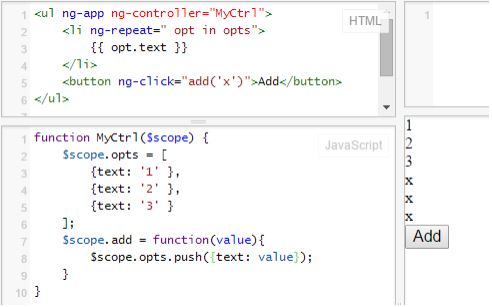
\includegraphics[width=1\textwidth]{figura34}
\caption{Exemplo de criação de nó com AngularJS.}
\end{figure}

\subsubsection{CSS}

O HTML5 possui atributos para personalizar as tags adicionadas, porém é um método depreciado e pouco eficiente com o surgimento do CSS3.

O CSS3 é uma linguagem de folha de estilo utilizada para definir a apresentação de documentos escritos em uma linguagem de marcação, como HTML5 e tem como papel principal separar o conteúdo de um documento e o seu formato.

A Figura 3.5 apresenta duas maneiras de como inserir personalizações CSS a um elemento: por classe e inline. A classe pode ser atribuída a vários elementos e assim todos terão apresentação em comum. Ao alterar uma classe, todos os elementos serão afetados e terão sua apresentação modificada. Os atributos da classe podem ser escritos no mesmo arquivo ou em um arquivo externo e importado. O método inline é adicionado com o “style”, é atribuído apenas ao elemento em questão e, caso haja alguma classe no elemento, sobrepõe os atributos coincidentes da classe.

\begin{figure}[!htb]
\centering
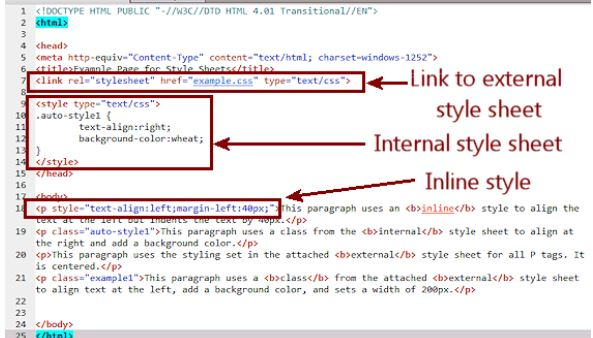
\includegraphics[width=1\textwidth]{figura35}
\caption{Métodos de utilização do CSS \url{http://bit.ly/1G00zSp}.}
\end{figure}


\subsection{LÓGICA DE PROGRAMAÇÃO}
\subsubsection{CONEXÃO COM BANCO DE DADOS}

Todo o conteúdo até o momento está do lado do cliente em JSON, não foi enviado nada para o servidor e não foi feita nenhuma persistência de informações, portanto as informações são perdidas ao fechar a aplicação. Para a conexão com o banco de dados foi utilizada a linguagem C\# da Microsoft, ela é uma linguagem orientada à objetos, fortemente tipada, foi baseada no C++ e possui similaridades com Java, linguagem desenvolvida em \textbf{Processamento da Informação, Programação Orientada a Objetos} e conceitos vistos em \textbf{Lógica Básica, Algoritmos e Estrutura de Dados e Análise de Algoritmos}.

A Figura 3.6 é um exemplo de conexão básica com o banco de dados na linguagem C\#
em que a conexão é declarada, em seguida são adicionados os parâmetros da conexão, a conexão é aberta, uma mensagem é exibida, a conexão é fechada e outra mensagem é exibida.

\begin{figure}[!htb]
\centering
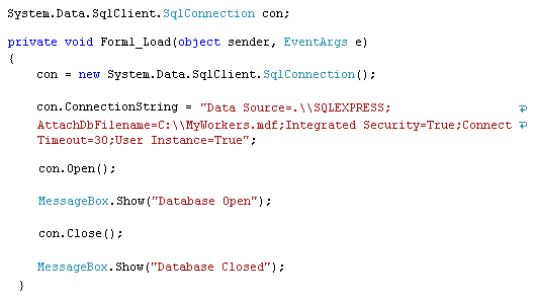
\includegraphics[width=1\textwidth]{figura36}
\caption{Exemplo de conexão básica com o bando de dados em C\#.}
\end{figure}



\subsubsection{EXPRESSÕES REGULARES}

Foram utilizadas expressões regulares, conteúdo de \textbf{Linguagens Formais e Autômata},
no Sistema de Bolsa de Estudos PROMAIS para verificar se os valores inseridos pelos usuários estavam de acordo com as informações necessárias, por exemplo: número de telefone não pode aceitar caracteres ou caracteres especiais, mas pode aceitar hífen, parênteses e espaço. Sendo assim, a expressão regular que representa uma maneira correta para telefone é exibida na Figura 3.7.

\begin{figure}[!htb]
\centering
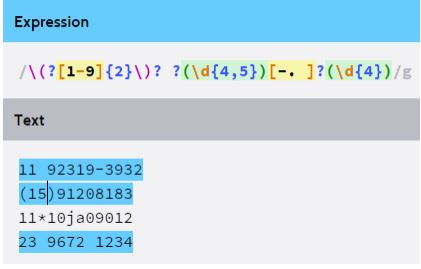
\includegraphics[width=0.7\textwidth]{figura37}
\caption{Expressão Regular para telefone.}
\end{figure}

Não há uma única expressão regular para alguns casos. Esse é um caso que depende da forma que o desenvolvedor decide para um melhor desempenho na sua aplicação. O exemplo apresentado permite receber telefones, obrigatoriamente, com DDD, mas sem obrigação dos parênteses. É permitido colocar espaço entre o DDD e o número ou preenchê-lo completamente sem espaço. No meio do telefone é aceito o sinal de hífen, ponto ou espaço. São aceitos telefones com oito ou nove números no total.



\subsection{BANCO DE DADOS}

Os bancos de dados de todas as aplicações foram desenvolvidos em SQL Server da Microsoft e a disciplina \textbf{Banco de Dados} instruiu os primeiros passos para desenvolver uma estrutura sólida e coerente, de acordo com as formas normais. A disciplina de\textbf{Segurança de Dados} também contribuiu para que as informações fossem transferidas de forma criptografada e segura de usuários não autorizados.

Com banco de dados é possível criar consultas específicas para retornar qualquer tipo de informação necessária pelo usuário. Tabelas podem ser relacionadas através das chaves primárias e estrangeiras. As chaves primárias representam uma identificação única para a informação e a chave estrangeira é a representação de uma informação de outra tabela. A Figura 3.8 apresenta o fluxo de uma consulta e os elementos possíveis, como: colunas a serem exibidas, as tabelas a serem consultadas, as condições de filtros, agrupamentos e filtros após os resultados.

\begin{figure}[!htb]
\centering
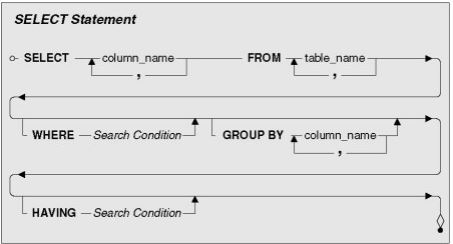
\includegraphics[width=0.7\textwidth]{figura38}
\caption{Modelo de consulta em banco de dados.}
\end{figure}
A modelagem dos bancos desenvolvidos pode ser vista em Figura 2.6 e Figura 2.14.
Nelas é possível notar que estão nas formas normais, existem relacionamentos “um para um”,
“um para n” e “n para n”.

Antes do desenvolvimento prático, foram feitas reuniões e modelagens conceituais para que fosse possível chegar ao modelo ideal sem que houvesse modificações durante o desenvolvimento das aplicações.


\section{CONSIDERAÇÕES FINAIS}
%%-- Conclusão do relatório, enfatizar os resultados a contribuição para a formação, dificuldades e futuras melhoras --%%


Este capítulo tem por objetivo descrever as contribuições que o estágio proporcionou à formação acadêmica e profissional, as dificuldades encontradas durante o processo e sugestões de trabalhos futuros.


\subsection{CONTRIBUIÇÕES PARA A FORMAÇÃO}

O estágio exigiu conhecimento e aplicação de várias disciplinas como Processamento da Informação, Programação para Web, Programação Orientada a Objetos, Banco de Dados, Lógica Básica, Computadores, Ética e Sociedade, Linguagens Formais e Autômata, Segurança de Dados, Programação para Dispositivos Móveis, Análise de Algoritmos e Engenharia de Software. O estágio exigiu o conhecimento para criar lógicas que solucionassem problemas,
operadores lógicos, expressões regulares, consultas em banco de dados, desenvolvimento em camadas (MVC) e planejamento.

As ferramentas ensinadas ao aluno durante os cursos de formação facilitaram as atividades e exigiram uma curva de aprendizado menor nos assuntos em que foi necessário aprofundamento, considerando que o aprendizado em um ambiente acadêmico acontece em um cenário ideal e pequeno em relação ao mercado de trabalho.

O período total foi suficiente para perceber a diferença entre a teoria e a prática. Na teoria todo o assunto é passado ao aluno, os conceitos, maneiras de resoluções de problemas, os exercícios e projetos são grandes desafios e são os que põem a prova tudo o que foi aprendido nas aulas, porém, quando o aluno se depara com a realidade do mercado de trabalho, nota a diferença da dimensão de tudo o que foi visto antes e que nas aulas, apesar de parecer um projeto grande, é apenas um pequeno exemplo que pode acontecer na realidade. Essa distância entre a teoria e a prática é o que amadurece e faz com que o estagiário aplique tudo o que foi aprendido, contribuindo no crescimento profissional.


\subsection{DIFICULDADES ENCONTRADAS}

O desenvolvimento de aplicações no ambiente de produção exige muita disciplina do profissional. O código deve ser bem estruturado, pois será mantido por uma equipe. Deve haver um planejamento do projeto antes de iniciar qualquer programação para evitar erros e trabalhos desnecessários. O profissional necessita pesquisar muito sobre como realizar a tarefa, qual seria a melhor solução, quais seriam as melhores ferramentas, conversar com outros desenvolvedores para adquirir experiência e criar uma solução ideal para o problema.

Algumas ferramentas utilizadas no decorrer do estágio não foram ensinadas nos cursos de formação do aluno, dificultando inicialmente o desenvolvimento dos projetos. Porém, tal fato implicou em um maior empenho e dedicação em estudos e pesquisas, gerando ótimos resultados nos projetos e amadurecendo o aluno profissionalmente.


\subsection{SUGESTÕES DE TRABALHOS FUTUROS}

As disciplinas ministradas aos alunos devem possuir uma reciclagem periodicamente,
pois a área de tecnologia possui novidades constantemente. Além da reciclagem nos assuntos de cada disciplina, também é preciso verificar a necessidade de novas disciplinas que possam abranger as novidades de hardware e/ou software.

Os projetos desenvolvidos pelo aluno possuem tecnologias e ferramentas recentes e esse caminho deve ser mantido. Foram utilizadas ferramentas de código aberto, que facilita a atualização por parte dos desenvolvedores e da comunidade que participa com constantes contribuições. Outras ferramentas e recursos podem ser agregados aos sistemas para facilitar a experiência do usuário, mas com cuidado para que não haja exageros e conflitos com as ferramentas atuais.

O AngularJS demonstrou ser uma ferramenta com pequena curva aprendizado para tarefas mais comuns em um sistema. Ele deve ser mantido e aperfeiçoado nos sistemas atuais ecotado para o desenvolvimento de novos sistemas.


\section{REFERÊNCIAS BIBLIOGRAFICAS}
%%-- Fontes utilizadas no relatório --%%

%%-- Indica-se o uso da bilioteca bibTEX--%%


[1] Tripletech, \url{http://www.tripletech.com.br/}, acessado em 03/08/2015 às 06h50

[2] Faculdade de Direito de São Bernardo do Campo, http://www.direitosbc.br/, acessado em 03/08/2015 às 07h00.

[3] Faculdade de Direito de São Bernardo do Campo - Bolsas de Estudos,

\url{http://www.direitosbc.br/a-faculdade-servicos-bolsa-de-estudo.aspx}, acessado em 04/08/2015 às 07h25.

[4] AngularJS by Google, \url{https://angularjs.org/}, acessado em 04/08/2015 às 07h40.

[5] JSON, \url{http://json.org/}, acessado em 04/08/2015 às 07h45.

[6] Bootstrap, \url{http://getbootstrap.com/}, acessado em 04/08/2015 às 08h15.

[7] Runrun.it, \url{http://runrun.it/}, acessado em 04/08/2015 às 13h20.

[8] Angular Material Design by Google,\url{ https://material.angularjs.org/latest/\#/}, acessado em 05/08/2015 às 13h50.

[9] Google, \url{http://google.com.br/}, acessado em 05/08/2015 às 13h55.

[10] Android 5.0 Lollipop,

\url{https://www.android.com/intl/pt-BR_br/versions/lollipop-5-0/},
acessado em 06/08/2015 às 07h35.

[11] Especificações Material Design by Google, https://www.google.com/design/spec/ material design/introduction.html, acessado em 06/08/2015 às 07h40.

[12] Google Inbox, \url{http://inbox.google.com.br/}, acessado em 06/08/2015 às 07h45.

[13] Google Music, \url{http://music.google.com.br/}, acessado em 06/08/2015 às 07h46.

[14] Google Keep, \url{http://keep.google.com.br/}, acessado em 06/08/2015 às 07h47.

[15] Sommerville, I. Engenharia de Software. 8.ed. - São Paulo : Addison-Wesley, 2007.

[16] Pressman, Roger S. Engenharia de Software. 6.ed. - Rio de Janeiro: McGraw-Hill, 2006

[17] O que é DOM, \url{http://tableless.com.br/tenha-o-dom/}, Acessado em 06/08/2015 às 13h35

\end{document}
